\documentclass[fleqn,10pt]{latex/stylish_article} % Document font size and equations flushed left

\setcounter{tocdepth}{3}

% Pandoc environments
\usepackage{framed}
\usepackage{fancyvrb}
\providecommand{\tightlist}{%
  \setlength{\itemsep}{0pt}\setlength{\parskip}{0pt}}
\newcommand{\VerbBar}{|}
\newcommand{\VERB}{\Verb[commandchars=\\\{\}]}
\DefineVerbatimEnvironment{Highlighting}{Verbatim}{commandchars=\\\{\}, fontsize=\scriptsize} % R Code

% Colored code
\usepackage{color}
\definecolor{shadecolor}{RGB}{248,248,248}
\newenvironment{Shaded}{\begin{snugshade}}{\end{snugshade}}
\newcommand{\KeywordTok}[1]{\textcolor[rgb]{0.13,0.29,0.53}{\textbf{{#1}}}}
\newcommand{\DataTypeTok}[1]{\textcolor[rgb]{0.13,0.29,0.53}{{#1}}}
\newcommand{\DecValTok}[1]{\textcolor[rgb]{0.00,0.00,0.81}{{#1}}}
\newcommand{\BaseNTok}[1]{\textcolor[rgb]{0.00,0.00,0.81}{{#1}}}
\newcommand{\FloatTok}[1]{\textcolor[rgb]{0.00,0.00,0.81}{{#1}}}
\newcommand{\ConstantTok}[1]{\textcolor[rgb]{0.00,0.00,0.00}{{#1}}}
\newcommand{\CharTok}[1]{\textcolor[rgb]{0.31,0.60,0.02}{{#1}}}
\newcommand{\SpecialCharTok}[1]{\textcolor[rgb]{0.00,0.00,0.00}{{#1}}}
\newcommand{\StringTok}[1]{\textcolor[rgb]{0.31,0.60,0.02}{{#1}}}
\newcommand{\VerbatimStringTok}[1]{\textcolor[rgb]{0.31,0.60,0.02}{{#1}}}
\newcommand{\SpecialStringTok}[1]{\textcolor[rgb]{0.31,0.60,0.02}{{#1}}}
\newcommand{\ImportTok}[1]{{#1}}
\newcommand{\CommentTok}[1]{\textcolor[rgb]{0.56,0.35,0.01}{\textit{{#1}}}}
\newcommand{\DocumentationTok}[1]{\textcolor[rgb]{0.56,0.35,0.01}{\textbf{\textit{{#1}}}}}
\newcommand{\AnnotationTok}[1]{\textcolor[rgb]{0.56,0.35,0.01}{\textbf{\textit{{#1}}}}}
\newcommand{\CommentVarTok}[1]{\textcolor[rgb]{0.56,0.35,0.01}{\textbf{\textit{{#1}}}}}
\newcommand{\OtherTok}[1]{\textcolor[rgb]{0.56,0.35,0.01}{{#1}}}
\newcommand{\FunctionTok}[1]{\textcolor[rgb]{0.00,0.00,0.00}{{#1}}}
\newcommand{\VariableTok}[1]{\textcolor[rgb]{0.00,0.00,0.00}{{#1}}}
\newcommand{\ControlFlowTok}[1]{\textcolor[rgb]{0.13,0.29,0.53}{\textbf{{#1}}}}
\newcommand{\OperatorTok}[1]{\textcolor[rgb]{0.81,0.36,0.00}{\textbf{{#1}}}}
\newcommand{\BuiltInTok}[1]{{#1}}
\newcommand{\ExtensionTok}[1]{{#1}}
\newcommand{\PreprocessorTok}[1]{\textcolor[rgb]{0.56,0.35,0.01}{\textit{{#1}}}}
\newcommand{\AttributeTok}[1]{\textcolor[rgb]{0.77,0.63,0.00}{{#1}}}
\newcommand{\RegionMarkerTok}[1]{{#1}}
\newcommand{\InformationTok}[1]{\textcolor[rgb]{0.56,0.35,0.01}{\textbf{\textit{{#1}}}}}
\newcommand{\WarningTok}[1]{\textcolor[rgb]{0.56,0.35,0.01}{\textbf{\textit{{#1}}}}}
\newcommand{\AlertTok}[1]{\textcolor[rgb]{0.94,0.16,0.16}{{#1}}}
\newcommand{\ErrorTok}[1]{\textcolor[rgb]{0.64,0.00,0.00}{\textbf{{#1}}}}
\newcommand{\NormalTok}[1]{{#1}}

% cslreferences environment required by pandoc > 2.7

% Polyglossia
\usepackage{polyglossia}
\setmainlanguage{en-US}

% localized quotes
\usepackage[strict,autostyle]{csquotes}

% Figures
\usepackage{graphicx,grffile}
\makeatletter
\def\maxwidth{\ifdim\Gin@nat@width>\linewidth\linewidth\else\Gin@nat@width\fi}
\def\maxheight{\ifdim\Gin@nat@height>\textheight0.8\textheight\else\Gin@nat@height\fi}
\makeatother
% Scale images if necessary, so that they will not overflow the page
% margins by default, and it is still possible to overwrite the defaults
% using explicit options in \includegraphics[width, height, ...]{}
\setkeys{Gin}{width=\maxwidth,height=\maxheight,keepaspectratio}

% Additional packages
\usepackage{natbib}             % Advanced Bibliography (citep...).
\usepackage{amsmath,amsfonts,amssymb}
\usepackage{breqn}              % Line breaks in equations
\usepackage{url}                % Line breaks in url's
\usepackage{enumitem}           % Line spacing in lists
  \setlist[itemize]{noitemsep,nolistsep}
  \setlist[enumerate]{noitemsep,nolistsep}

% Tables
\usepackage{longtable,booktabs}
\usepackage{caption}
% These lines are needed to make table captions work with longtable:
\makeatletter
\def\fnum@table{\tablename~\thetable}
\makeatother
% longtable 2 columns
% https://tex.stackexchange.com/questions/161431/how-to-solve-longtable-is-not-in-1-column-mode-error
\makeatletter
\let\oldlt\longtable
\let\endoldlt\endlongtable
\def\longtable{\@ifnextchar[\longtable@i \longtable@ii}
\def\longtable@i[#1]{\begin{figure}[t]
\onecolumn
\begin{minipage}{0.5\textwidth}\scriptsize
\oldlt[#1]
}
\def\longtable@ii{\begin{figure}[t]
\onecolumn
\begin{minipage}{0.5\textwidth}\scriptsize
\oldlt
}
\def\endlongtable{\endoldlt
\end{minipage}
\twocolumn
\end{figure}}
\makeatother

% Full-width tables
\usepackage{tabu}
\renewenvironment{table}{\begin{table*}}{\end{table*}\ignorespacesafterend}

% Prevent overfull lines
\setlength{\emergencystretch}{3em}

% User-adder preamble
\hyphenation{quan-tile re-gres-sion out-li-ers het-ero-ske-das-tic}

% hyperref comes last
\usepackage{hyperref}           % Hypertext links, PDF bookmarks
  \hypersetup{%
    urlcolor=blue,%
    linkcolor=black,citecolor=black,colorlinks=true%
  }

%----------------------------------------------------------------------------------------
%	ARTICLE INFORMATION
%----------------------------------------------------------------------------------------

\JournalInfo{\ }
\Archive{\ }

\PaperTitle{Advance Regression Term Project} % Article title

\Authors{
Gerard Palomo \& Juan Pablo Uphoff\textsuperscript{}
} % Authors
\affiliation{

}
\affiliation{*\textbf{}: } % Corresponding author

\Keywords{Quantile Regression, Robustness, Heteroscedasticity, OLS, Outliers} % Keywords
\newcommand{\keywordname}{Keywords} % Defines the keywords heading name

\JEL{C15, C21} % JEL codes
\newcommand{\JELname}{} % Defines the JEL heading name

\Acknowledgements{This report was completed for the course \textbf{Advanced Regression and Prediction}, as part of the \textbf{MSc in Statistics for Data Science} at \textbf{University Carlos III of Madrid}.} % Acknowledgements
\newcommand{\acknowledgementsname}{} % Defines the heading name

%----------------------------------------------------------------------------------------
%	ABSTRACT
%----------------------------------------------------------------------------------------

\Abstract{
Linear quantile regression (QR) extends ordinary least squares (OLS) by modeling conditional quantiles, offering a richer view of the response variable's distribution beyond the conditional mean provided by OLS. This paper highlights two key advantages of QR over OLS. Firstly, QR provides robustness to outliers in the response variable, a significant limitation for OLS which relies on minimizing squared errors. Secondly, QR allows for modeling distributional heterogeneity, such as heteroscedasticity, which OLS inherently overlooks by focusing solely on the mean. We compare the performance of OLS and linear QR estimators through a simulation study in a univariate setting. We examine performance under three conditions: (1) a baseline scenario with homoscedastic Gaussian errors, (2) contamination where outliers are introduced at high-leverage points to assess robustness, and (3) heteroscedastic errors to assess distributional modeling capabilities. We specifically compare OLS with QR at the 0.1, 0.5 (median), and 0.9 quantiles. Key performance metrics, including Mean Absolute Error (MAE) and coefficient stability, are assessed. Results demonstrate that QR estimates, particularly the median (\(\tau=0.5\)), remain reliable under outlier contamination where OLS estimates become significantly biased. Furthermore, QR effectively captures distributional effects like heteroscedasticity, providing quantile-specific insights that OLS cannot. All simulation code is provided in R for reproducibility.
}

%----------------------------------------------------------------------------------------

\begin{document}

\selectlanguage{en-US}

\flushbottom % Makes all text pages the same height

\maketitle % Print the title and abstract box

\tableofcontents % Print the contents section

\thispagestyle{empty} % Removes page numbering from the first page

%----------------------------------------------------------------------------------------
%	ARTICLE CONTENTS
%----------------------------------------------------------------------------------------

\section{Introduction}\label{introduction}

Classical linear regression, estimated via ordinary least squares (OLS), focuses on modeling the conditional mean of a response variable by minimizing the sum of squared residuals. While powerful under ideal assumptions, OLS faces significant limitations in practice. Its reliance on squared errors renders estimates highly sensitive to outliers, potentially leading to biased results. Furthermore, OLS provides only a partial view of the conditional distribution by focusing solely on the central tendency and typically assumes homoscedastic errors, limiting its ability to describe relationships where the variability of the response changes with predictors.

Quantile regression (QR), introduced by Koenker and Bassett (1978), offers a more comprehensive and robust alternative. By modeling conditional quantiles (e.g., the median, quartiles, deciles), QR addresses the shortcomings of OLS in two crucial ways. First, its estimation, based on minimizing an asymmetrically weighted sum of absolute errors (the check loss function), provides inherent robustness against outliers in the response variable; the influence of extreme observations is bounded, unlike in OLS. Prior studies, such as John (2015), have confirmed the superior performance of quantile regression over OLS in the presence of outliers. Second, QR provides a mechanism to characterize the entire conditional distribution of the response variable, not just its mean. This allows researchers to understand how predictors affect different parts of the distribution, making it particularly well-suited for analyzing data with heteroscedasticity or other forms of distributional heterogeneity.

This report aims to compare the performance of OLS and linear quantile regression estimators, focusing on these two key advantages of QR. We will demonstrate the robustness advantage of QR, particularly the conditional median (\(\tau=0.5\)), under controlled outlier contamination in a simple linear model, contrasting it with the sensitivity of OLS. Additionally, we will illustrate QR's ability to capture distributional heterogeneity by examining its performance under heteroscedastic errors, showcasing how it provides insights beyond the conditional mean estimated by OLS. We conduct a simulation study designed to highlight these differences visually and quantitatively, examining estimator behavior under three distinct scenarios: (1) a baseline homoscedastic Gaussian setting, (2) the same setting contaminated with high-leverage outliers, and (3) a setting with heteroscedastic errors. Coefficient stability and prediction accuracy (using Mean Absolute Error) are assessed across these scenarios.

\section{Linear Quantile Regression: Theory and Methods}\label{linear-quantile-regression-theory-and-methods}

\subsection{Definition and Estimation}\label{definition-and-estimation}

For a random variable \(Y\), the \(\tau\)-th quantile is the value \(q_\tau\) such that \(P(Y \le q_\tau) = \tau\). In a regression setting, quantile regression (QR) estimates:

\[
Q_Y(\tau \mid X = x) = x^\top \beta(\tau),
\]

where \(\beta(\tau)\) is a vector of coefficients specific to quantile level \(\tau\). For example, \(\beta_1(0.5)\) represents the effect of \(X_1\) on the median of \(Y\).

Koenker and Bassett (1978) proposed estimating \(\beta(\tau)\) by minimizing the check loss:

\[
\hat\beta(\tau) = \arg\min_\beta \sum_{i=1}^n \rho_\tau(y_i - x_i^\top \beta),
\]

with \(\rho_\tau(u) = u(\tau - \mathbb{I}\{u < 0\})\). For \(\tau = 0.5\), this reduces to least absolute deviations (LAD) regression.

Each \(\tau\) is estimated independently using linear programming, and the family \(\{\beta(\tau)\}\) forms a quantile process describing the full conditional distribution of \(Y\).

\subsection{Inference}\label{inference}

Under regularity conditions, \(\hat\beta(\tau)\) is asymptotically normal:

\[
\sqrt{n}(\hat\beta(\tau) - \beta(\tau)) \overset{d}{\to} N(0, \Sigma(\tau)),
\]

with variance estimators obtained via bootstrapping or sandwich estimators (Koenker, 2005). Practical inference is available via \texttt{summary()} in the R package \texttt{quantreg}.

\subsection{Comparison to OLS}\label{comparison-to-ols}

OLS estimates the conditional mean:

\[
\mathbb{E}[Y \mid X = x] = x^\top \beta,
\]

whereas QR estimates conditional quantiles. When errors are symmetric and homoscedastic, QR and OLS give similar results. Otherwise, QR captures distributional heterogeneity, such as increasing variance or skewness.

Moreover, QR is robust to outliers in \(Y\), unlike OLS which minimizes squared error and is sensitive to extreme values. QR also allows different slopes across quantiles, offering richer interpretation.

In the next section, we illustrate these theoretical advantages through a simulation study.

\section{Simulation Study}\label{simulation-study}

This section presents a simulation study designed to compare the performance of \textbf{Ordinary Least Squares (OLS)} and \textbf{Quantile Regression (QR)} estimators under controlled, interpretable scenarios. Our aim is to assess how both methods behave, particularly under outlier contamination and additionally under heteroscedasticity.

To focus on the theoretical properties discussed in Section 2, we restrict attention to a simple univariate linear model with a single predictor. This allows for clean interpretation and visual representation of the results. Additionally, we consider three error structures: a baseline homoscedastic Gaussian case, a contaminated version with outliers at high-leverage points and a heteroscedastic case. This controlled setup isolates the impact of extreme observations on both methods, and is helps to reveal the key differences in robustness and sensitivity.

\subsection{Data Generating Process (DGP)}\label{data-generating-process-dgp}

We consider the simple linear model \(Y = \beta_0 + \beta_1 X_1 + \varepsilon\), with fixed parameters \(\beta_0 = 5\) and \(\beta_1 = -1.5\). These values are chosen to induce a moderate negative slope and an interpretable intercept, ensuring that both OLS and QR coefficients remain in a tractable range for interpretation and graphical analysis. The predictor \(X_1\) is generated from a uniform distribution on \([0,10]\), which provides a constant density across its support and avoids introducing implicit bias or skewness into the covariate structure. The sample size \(n = 1000\) is selected to approximate asymptotic behavior while remaining computationally feasible. While we compute QR estimates for multiple quantiles (\(\tau \in \{0.1, 0.5, 0.9\}\)), the primary focus is on \(\tau = 0.5\), which corresponds to the conditional median and allows direct comparison with the OLS estimator of the conditional mean. As highlighted in Section 2, QR estimates \(\beta(\tau)\) independently for each \(\tau\), thus providing a richer description of the conditional distribution of \(Y\) than OLS.

\subsection{Simulation Setup}\label{simulation-setup}

To evaluate the estimators under different conditions relevant to their theoretical properties, we simulate data using the DGP described above under three distinct error structures for \(\varepsilon\):

\begin{enumerate}
\def\labelenumi{\arabic{enumi}.}
\item
  \textbf{Baseline Homoscedastic Gaussian Errors:} We first consider \(\varepsilon_i \sim \mathcal{N}(0, \sigma^2)\) with a constant variance \(\sigma = 2\). This scenario satisfies the classical OLS assumptions and serves as a benchmark for comparing OLS and QR under ideal conditions.
\item
  \textbf{Contaminated Gaussian Errors (Outlier Robustness Test):} To assess robustness, we start with the baseline homoscedastic Gaussian errors and introduce contamination. Specifically, 2\% of the observations (\(n \times 0.02\)) with the largest values of the predictor \(X_1\) (high-leverage points) have their corresponding error terms perturbed by a large positive constant (\(+50\)). This creates vertical outliers combined with leverage, designed to maximally challenge the estimators' stability.
\item
  \textbf{Heteroscedastic Gaussian Errors (Distributional Modeling Test):} To illustrate the ability of QR to model distributional heterogeneity, we simulate errors whose variance increases linearly with the predictor: \(\varepsilon_i \sim \mathcal{N}(0, \sigma_i^2)\), where \(\sigma_i = \sigma_0 (1 + \gamma X_{1i})\). We use parameters like \(\sigma_0 = 1\) and \(\gamma = 0.3\) to generate noticeable heteroscedasticity. This scenario violates the OLS assumption of constant variance.
\end{enumerate}

For each scenario, we fit both the OLS model and QR models at \(\tau \in \{0.1, 0.5, 0.9\}\).

\subsection{Evaluation Metrics}\label{evaluation-metrics}

To quantify the behavior of the estimators, we combine visual inspection with numerical performance metrics. Given that QR minimizes absolute deviations, particularly for \(\tau = 0.5\), we employ the \textbf{Mean Absolute Error (MAE)} as the primary metric. MAE is defined as \(\text{MAE} = \frac{1}{n} \sum_{i=1}^n |y_i - \hat{y}_i|\), and aligns directly with the objective function of the LAD estimator. It provides a robust measure of predictive accuracy and is less sensitive to outliers than the \textbf{RMSE}, which disproportionately penalizes large deviations. This makes MAE more appropriate when comparing methods under contamination or heavy-tailed noise, as discussed by Koenker (2005).

\subsection{Simulation}\label{simulation}

We now illustrate the theoretical differences between OLS and quantile regression through a basic univariate simulation. Using the data-generating process defined in Section 3.1, we compare both estimators under clean and contaminated conditions. We focus on the conditional median estimate (QR at \(\tau = 0.5\)) and examine how each method responds to the presence of vertical outliers in high-leverage positions.

As shown in the figure @ref(fig:slope\_plot), both OLS (dashed red line) and quantile regression (blue line) yield nearly identical slope estimates when applied to clean, homoscedastic data. This is in line with the theoretical results discussed in Section 2.3, where OLS and QR coincide under symmetric and homoscedastic error distributions. However, under contamination, even with as little as 2\% of vertical outliers placed at high-leverage points, the OLS slope is visibly distorted---flattening as it attempts to minimize squared error. In contrast, the QR line remains largely unaffected, producing a slope estimate that better reflects the central structure of the data. This illustrates the robustness property of quantile regression highlighted earlier: since QR minimizes a weighted absolute loss, it is less sensitive to large deviations in the response, and more resilient to local anomalies.

\begin{figure}

{\centering 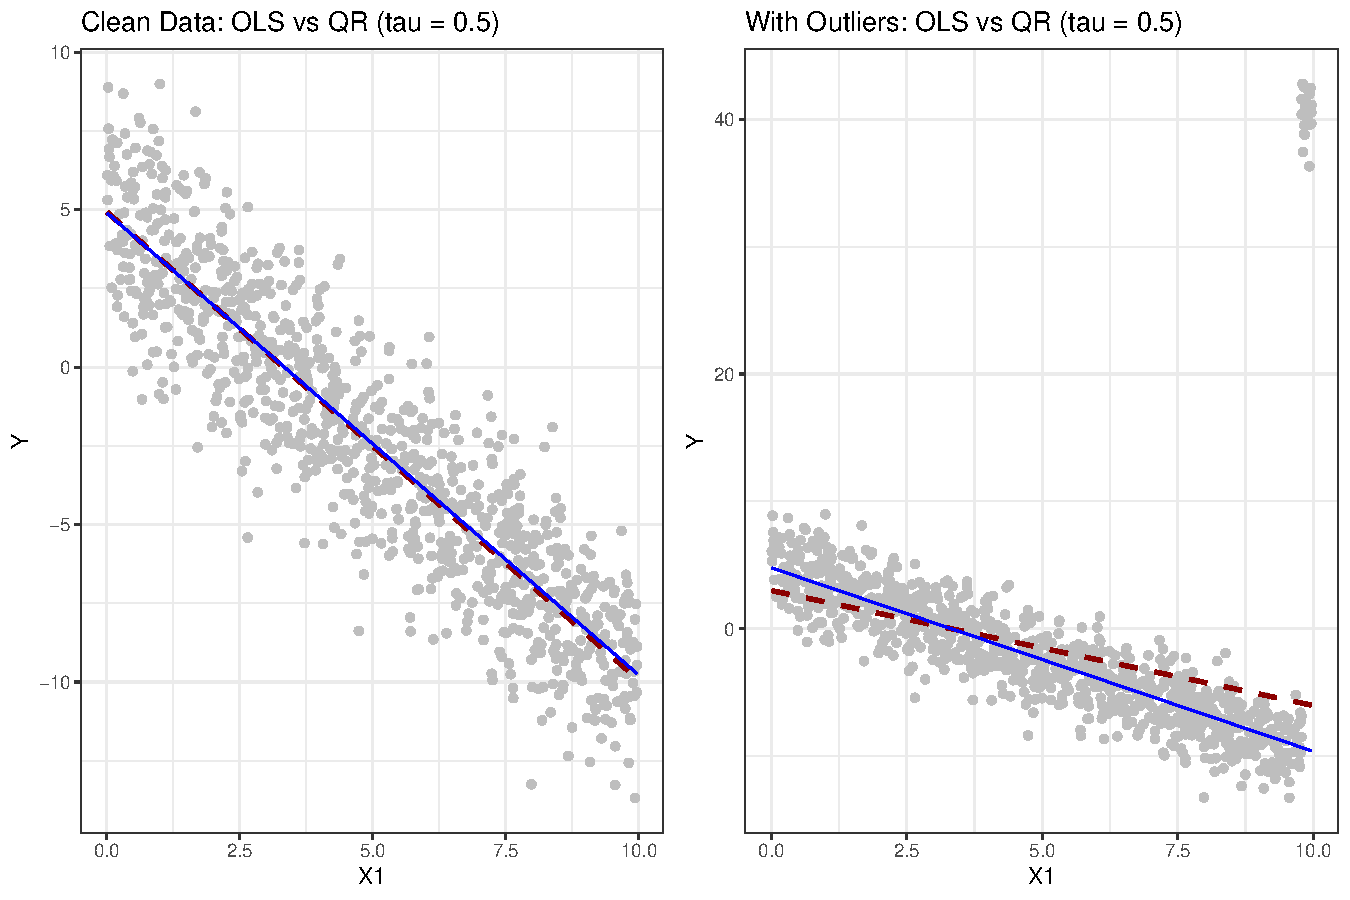
\includegraphics[width=0.8\linewidth]{ADR_project_draft_files/figure-latex/slope_plot-1} 

}

\caption{Comparison of slope estimates across settings}(\#fig:slope_plot)
\end{figure}

\begin{table}[!h]
\centering
\caption{(\#tab:sum_table)OLS vs Quantile Regression Coefficient Comparison}
\centering
\begin{tabular}[t]{lrrrr}
\toprule
Coefficient & OLS\_Clean & QR\_Clean & OLS\_Outliers & QR\_Outliers\\
\midrule
(Intercept) & 4.931 & 4.903 & 3.004 & 4.791\\
X1 & -1.487 & -1.468 & -0.903 & -1.442\\
\bottomrule
\end{tabular}
\end{table}

Figure @ref(fig:slope\_quantile) illustrates how the estimated slope coefficient in quantile regression varies across quantile levels \(\tau \in (0.05, 0.95)\) in a heteroskedastic setting. The increasing trend in slope estimates as \(\tau\) increases reflects the presence of conditional heteroskedasticity: higher quantiles are associated with greater dispersion in the response variable \(Y\), which alters the marginal effect of \(X_1\) across the conditional distribution.

The dashed red line represents the OLS slope, which remains constant because it targets the conditional mean and assumes homoscedasticity. In contrast, quantile regression estimates \(\beta_1(\tau)\) independently for each \(\tau\), capturing variation in the conditional distribution of \(Y\).

\begin{figure}

{\centering 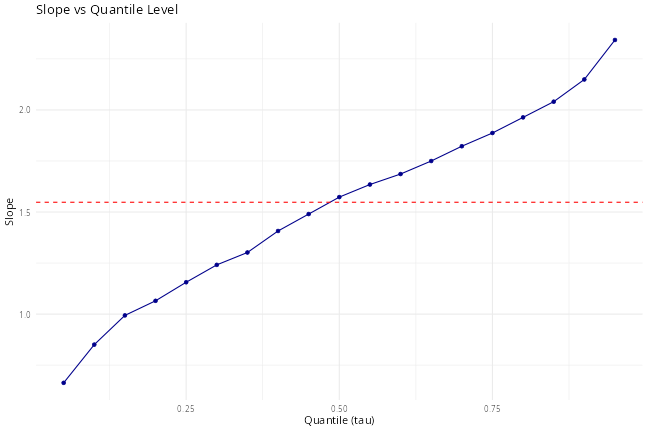
\includegraphics[width=0.8\linewidth]{ADR_project_draft_files/figure-latex/slope_quantile-1} 

}

\caption{Slope vs Quantile for heteroskedastic data}(\#fig:slope_quantile)
\end{figure}

Figure @ref(fig:other\_plots) presents a multifaceted comparison between OLS and quantile regression under heteroskedasticity and contamination. In the top-left panel, QR lines at \(\tau = 0.1, 0.5, 0.9\) capture the conditional distributional spread of \(Y\), while OLS fits a single conditional mean. The top-right panel plots the estimated slope \(\beta_1(\tau)\) across quantiles. The non-constant pattern confirms that the marginal effect of \(X\) varies with \(\tau\), violating the constant-slope assumption implicit in OLS, as discussed in Section 2.3.

The bottom-left panel illustrates robustness: under contamination, OLS is pulled downward due to extreme values in \(Y\), while the median QR line remains stable. Finally, the residual histograms (bottom-right) show that OLS residuals are more dispersed and asymmetric, reflecting its sensitivity to outliers, whereas QR residuals remain more concentrated.

\begin{figure}

{\centering 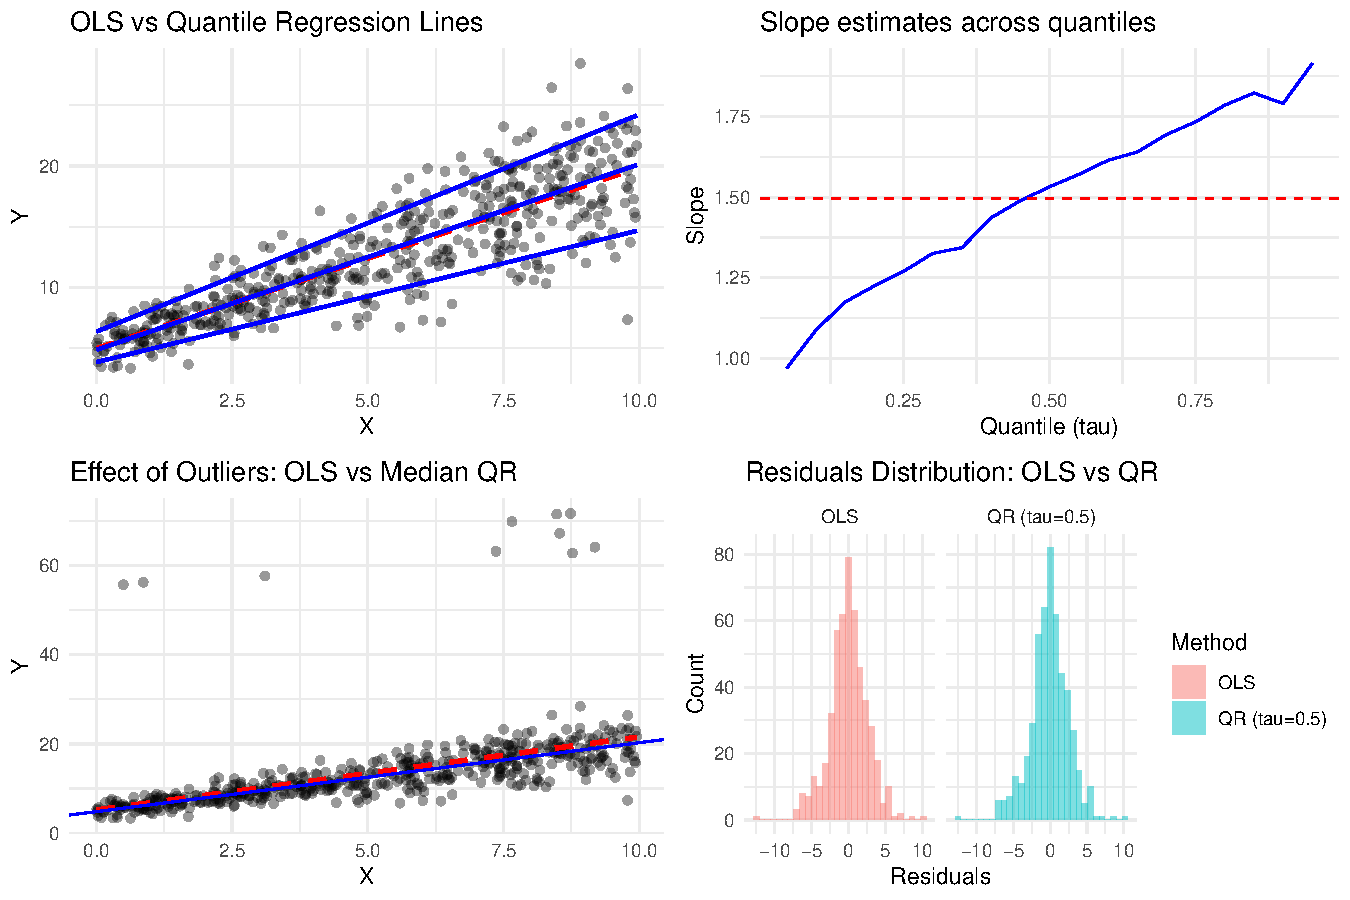
\includegraphics[width=0.8\linewidth]{ADR_project_draft_files/figure-latex/other_plots-1} 

}

\caption{Slope vs Quantile for heteroskedastic data}(\#fig:other_plots)
\end{figure}

Table @ref(tab:eval\_table) illustrates the comparative robustness of OLS and quantile regression (QR at \(\tau = 0.5\) under clean and contaminated settings. Both estimators perform similarly in the Gaussian case. However, under contamination, OLS coefficients exhibit severe bias, particularly in the slope, while QR remains stable. This behavior is theoretically consistent with QR's bounded influence function and its minimization of the check loss, which limits sensitivity to extreme values. MAE, aligned with the LAD objective, remains nearly unchanged for QR, whereas OLS shows substantial deterioration. RMSE, although not optimized by QR, is included for standard comparison and further confirms OLS's vulnerability under outlier contamination.

\begin{table}[!h]
\centering
\caption{(\#tab:metrics_table, echoFALSE)OLS vs Quantile Regression: Coefficients and Error Metrics under Different Error Structures}
\centering
\begin{tabular}[t]{lllrrrrr}
\toprule
  & Model & Method & Intercept & Slope & Slope\_Bias & MAE & RMSE\\
\midrule
(Intercept)...1 & Gaussian & QR & 4.903 & -1.468 & 0.032 & 1.533 & 1.925\\
(Intercept)...2 & Contaminated & QR & 4.791 & -1.442 & 0.058 & 1.534 & 1.930\\
(Intercept)...3 & Gaussian & OLS & 4.931 & -1.487 & 0.013 & 1.534 & 1.924\\
(Intercept)...4 & Contaminated & OLS & 3.004 & -0.903 & 0.597 & 2.229 & 2.746\\
\bottomrule
\end{tabular}
\end{table}

Figure @ref(fig:slope\_outliers) shows the evolution of the estimated slope \(\hat{\beta}_1\) as a function of outlier contamination. As predicted by the robustness theory in Section 2.3, QR remains stable under moderate contamination, exhibiting high resistance to leverage-induced distortion. However, once the proportion of outliers exceeds a critical threshold (\textasciitilde25\%), their influence becomes structurally dominant---shifting the conditional median itself and leading to breakdown. In contrast, OLS degrades continuously, with no resistance to contamination at any level.

\begin{figure}

{\centering 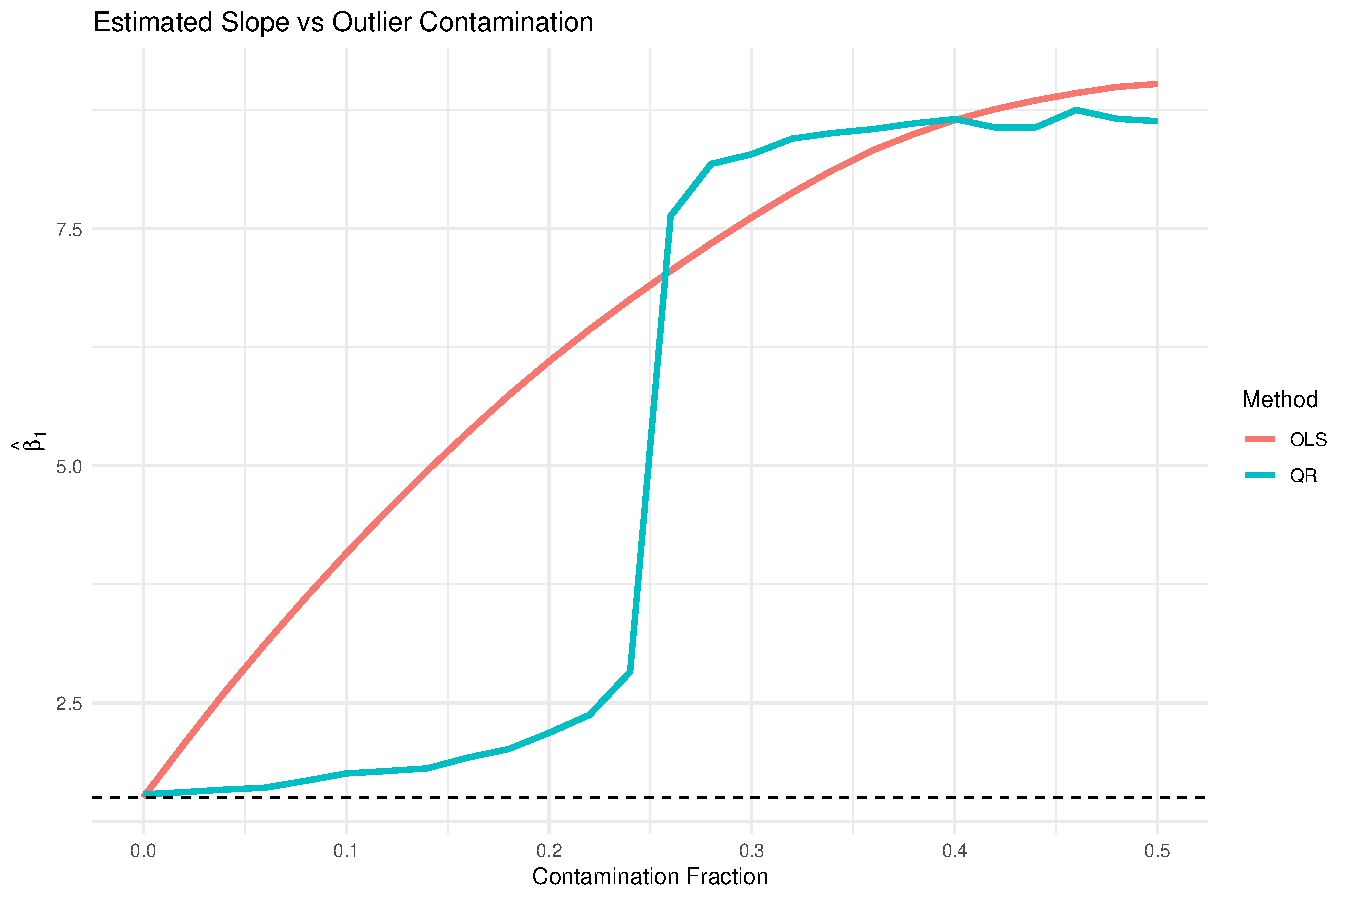
\includegraphics[width=0.8\linewidth]{ADR_project_draft_files/figure-latex/slope_outliers-1} 

}

\caption{Estimated slope vs outlier contamination}(\#fig:slope_outliers)
\end{figure}

\section{Discussion \& Conclusions}\label{discussion-conclusions}

This report has compared ordinary least squares (OLS) and quantile regression (QR) for modeling linear relationships, focusing on scenarios where classical OLS assumptions are violated. Through controlled simulations, we demonstrated two primary advantages of QR. Firstly, QR, particularly median regression (\(\tau=0.5\)\$, exhibits significant \textbf{robustness to outliers}, providing stable and reliable coefficient estimates even under contamination with high-leverage points, a condition where OLS estimates suffered severe bias (as shown in Figure @ref(fig:slope\_plot) and Table @ref(tab:eval\_table)). This resilience stems from QR's use of the check loss function, which minimizes absolute deviations rather than squared deviations.

Secondly, QR offers a powerful tool for characterizing \textbf{distributional heterogeneity}. Our simulations under heteroscedastic errors (Figures @ref(fig:slope\_quantile) and @ref(fig:other\_plots)) showed that QR can effectively capture how the effect of predictors varies across different quantiles of the response distribution, revealing patterns (like increasing variance) that are entirely missed by the single conditional mean estimate provided by OLS. The quantile-specific slopes provide a richer, more nuanced understanding of the underlying data generating process.

In conclusion, while OLS remains a cornerstone of regression analysis, quantile regression provides a flexible, robust, and more informative alternative, particularly valuable when dealing with non-Gaussian errors, outliers, or heteroscedasticity. These results highlight its utility as a complementary, and often superior, tool for modeling complex data relationships.

\textbf{Considerations}: \textbf{\emph{This report has been made with a template in R Markdown. CHATGPT has been used for cleaning the code and debugging.}}

%----------------------------------------------------------------------------------------
%	REFERENCE LIST
%----------------------------------------------------------------------------------------

\bibliographystyle{apalike}
\makeatletter
% The filename has .bib extension that must be eliminated
\filename@parse{references.bib}
% parse stores the file name in base. Extension starts at the first dot, so don't use dots in file names.
\bibliography{\filename@base}
\makeatother


%----------------------------------------------------------------------------------------

\end{document}
